% =====================================================================
%  Proposal presentation (Beamer, single-file)
%  Predicting the Zero-Shot Transfer of a Promptable Video Tracker
%  Build:  report/build.sh presentation   (Tectonic + Ghostscript-normalise)
% =====================================================================
\documentclass[aspectratio=169,11pt]{beamer}
\usetheme{default}
\setbeamertemplate{navigation symbols}{}
\setbeamertemplate{footline}[frame number]
\setbeamertemplate{itemize items}[circle]

\usepackage{amsmath}
\usepackage{booktabs}
\usepackage{tikz}
\usetikzlibrary{positioning,arrows.meta,calc}

% --- self-contained palette (no dvipsnames dependency) ---
\definecolor{navy}{RGB}{30,64,124}
\definecolor{forest}{RGB}{34,120,60}
\definecolor{burnt}{RGB}{214,104,26}
\definecolor{plum}{RGB}{140,55,135}
\setbeamercolor{structure}{fg=navy}
\setbeamercolor{frametitle}{fg=navy}
\setbeamerfont{frametitle}{series=\bfseries}

\newcommand{\frozen}[1]{{\color{navy}\textbf{#1}}}

\title[Predicting Zero-Shot Transfer]{Predicting the Zero-Shot Transfer\\of a Promptable Video Tracker}
\subtitle{Forecasting SAM\,3's reliability on unseen species \& places --- from label-free distances}
\author{Kostiantyn Boiar}
\institute{MSc Thesis Proposal \,\textbullet\, University of Glasgow\\[2pt]
\small Supervisor: Dr Marwa Mahmoud}
\date{\today}

\begin{document}

% ---------------------------------------------------------------- title
\begin{frame}[plain]
  \titlepage
\end{frame}

% ------------------------------------------------------------ the problem
\begin{frame}{The problem}
  \begin{block}{}
    \centering\large
    Promptable trackers (\textbf{SAM\,3}) segment \& track \emph{any} named animal in a video with
    \textbf{no training on that species}.
  \end{block}
  \vspace{0.6em}
  \begin{itemize}
    \item Conservation teams point them at new species / regions \textbf{constantly}.
    \item But nobody can say \emph{in advance} whether the model is \textbf{trustworthy} for a given
          animal in a given place.
    \item There is \textbf{no rule} that predicts this. That gap is what we fill.
  \end{itemize}
\end{frame}

% ------------------------------------------------------------ the question
\begin{frame}{The question}
  \begin{block}{}
    \centering\large
    Can we predict SAM\,3's zero-shot accuracy on an \textbf{unseen (species, place)}
    \emph{before running it} --- from properties measurable in advance?
  \end{block}
  \vspace{0.6em}
  \begin{itemize}
    \item \textbf{Not} trying to make the tracker score higher --- we predict \& explain its reliability.
    \item And: \emph{which factors} govern transfer, separately for \textbf{finding} the animal and
          \textbf{following} it?
  \end{itemize}
\end{frame}

% --------------------------------------------------------- metric decomposes
\begin{frame}{The metric decomposes --- and that is the point}
  \centering
  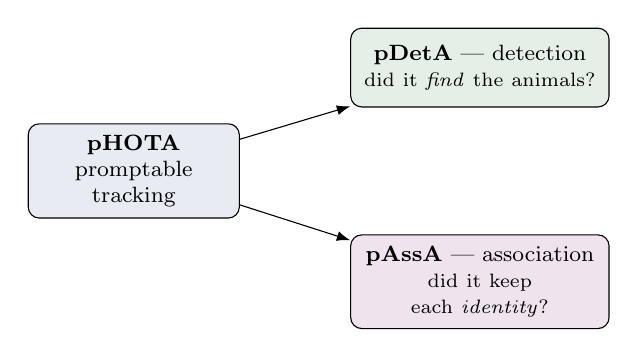
\begin{tikzpicture}[>=Latex,
    box/.style={draw,rounded corners,align=center,font=\footnotesize,inner sep=4pt,minimum height=1cm}]
    \node[box,fill=navy!10,text width=2.4cm] (h) {\textbf{pHOTA}\\promptable tracking};
    \node[box,fill=forest!12,text width=3.0cm,above right=0.2cm and 1.4cm of h] (d)
        {\textbf{pDetA} --- detection\\\scriptsize did it \emph{find} the animals?};
    \node[box,fill=plum!14,text width=3.0cm,below right=0.2cm and 1.4cm of h] (a)
        {\textbf{pAssA} --- association\\\scriptsize did it keep each \emph{identity}?};
    \draw[->] (h) -- (d); \draw[->] (h) -- (a);
  \end{tikzpicture}

  \vspace{0.6em}
  \footnotesize We analyse the \textbf{two components separately} (HOTA-style) --- the hypothesis is
  they transfer for \emph{different reasons}.
\end{frame}

% ------------------------------------------------------------ hypotheses
\begin{frame}{Hypotheses}
  \begin{block}{}\centering\footnotesize
    \textbf{H0 (null):} the label-free distances carry \emph{no} predictive signal --- transfer isn't
    distance-driven.\; H1/H2 are the directional alternatives:
  \end{block}
  \vspace{0.3em}
  \centering
  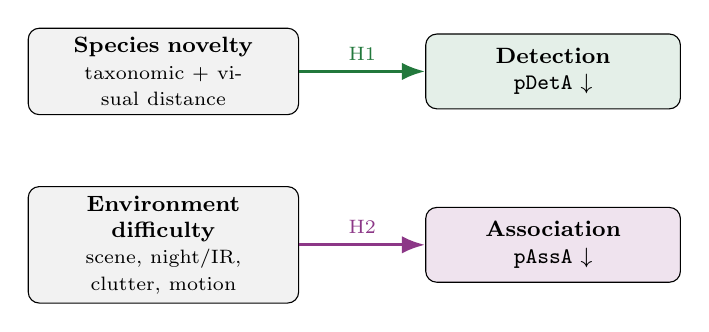
\begin{tikzpicture}[>=Latex,
    src/.style={draw,rounded corners,fill=black!5,align=center,font=\footnotesize,text width=3.2cm,minimum height=0.95cm},
    tgt/.style={draw,rounded corners,align=center,font=\footnotesize,text width=3.0cm,minimum height=0.95cm}]
    \node[src] (sn) {\textbf{Species novelty}\\\scriptsize taxonomic + visual distance};
    \node[tgt,fill=forest!12,right=1.6cm of sn] (det) {\textbf{Detection}\\\texttt{pDetA} $\downarrow$};
    \node[src,below=0.9cm of sn] (env) {\textbf{Environment difficulty}\\\scriptsize scene, night/IR, clutter, motion};
    \node[tgt,fill=plum!14,right=1.6cm of env] (ass) {\textbf{Association}\\\texttt{pAssA} $\downarrow$};
    \draw[->,forest,very thick] (sn)--(det) node[midway,above,font=\scriptsize]{H1};
    \draw[->,plum,very thick] (env)--(ass) node[midway,above,font=\scriptsize]{H2};
  \end{tikzpicture}

  \vspace{0.4em}
  \footnotesize Failing to reject H0 is itself a result --- it motivates a pivot to representational probing.
\end{frame}

% ------------------------------------------------------------ the data
\begin{frame}{The data --- SA-FARI: a natural experiment}
  \begin{itemize}
    \item Largest open multi-animal wildlife tracking set (Meta $\times$ Conservation X Labs).
    \item \textbf{99 species} (full 7-level taxonomy) $\cdot$ \textbf{741 locations} / 4 continents
          $\cdot$ a decade of footage.
    \item \textbf{Train / test disjoint by species \emph{and} location} $\Rightarrow$ every test video is
          a \emph{controlled probe} of transfer along a measurable distance.
    \item Hard negatives (query returns nothing) are \textbf{kept} --- they drive false-positive analysis.
  \end{itemize}
  \vspace{0.3em}
  \begin{block}{}
    \centering Species $\times$ place $\times$ time $=$ the axes we measure distance along.
  \end{block}
\end{frame}

% ------------------------------------------------------------ approach
\begin{frame}{Approach --- freeze the model, fit a small law}
  \centering
  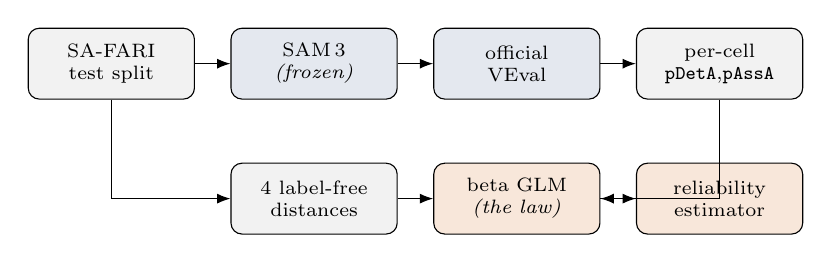
\begin{tikzpicture}[>=Latex,
    box/.style={draw,rounded corners,align=center,font=\scriptsize,inner sep=3pt,text width=1.9cm,minimum height=0.9cm}]
    \node[box,fill=black!5] (saf) {SA-FARI\\test split};
    \node[box,fill=navy!12,right=0.45cm of saf] (sam) {SAM\,3\\\textit{(frozen)}};
    \node[box,fill=navy!12,right=0.45cm of sam] (vev) {official\\VEval};
    \node[box,fill=black!5,right=0.45cm of vev] (sco) {per-cell\\\texttt{pDetA},\texttt{pAssA}};
    \node[box,fill=black!5,below=0.8cm of sam] (dist) {4 label-free\\distances};
    \node[box,fill=burnt!16,below=0.8cm of vev] (law) {beta GLM\\\textit{(the law)}};
    \node[box,fill=burnt!16,right=0.45cm of law] (rel) {reliability\\estimator};
    \draw[->] (saf)--(sam); \draw[->] (sam)--(vev); \draw[->] (vev)--(sco);
    \draw[->] (saf.south) |- (dist.west);
    \draw[->] (dist)--(law); \draw[->] (sco) |- (law.east);
    \draw[->] (law)--(rel);
  \end{tikzpicture}

  \vspace{0.5em}
  \footnotesize SAM\,3 \frozen{frozen}; the metric is the \textbf{official} one. Only the small
  \frozen{beta GLM} is fit --- from label-free distances. \textbf{No target label enters a distance.}
\end{frame}

% ------------------------------------------------------------ distances
\begin{frame}{The four label-free distances (+ a proxy)}
  \begin{itemize}
    \item \textbf{Taxonomic} --- tree steps to the nearest training species (lowest common ancestor).
    \item \textbf{Visual} --- DINOv2 embedding of the \emph{mask-cropped} animal vs.\ nearest training
          prototype (CLIP variant as a robustness check).
    \item \textbf{Environment} --- scene embedding of the masked-out background vs.\ nearest training
          location; $+$ a night/IR flag.
    \item \textbf{Temporal} --- years to the nearest relevant training footage.
    \item \textbf{SAM-3 familiarity proxy} --- separability in SAM\,3's \emph{own} feature space (hedges
          the unknown pretraining set).
  \end{itemize}
  \vspace{0.2em}
  \centering\footnotesize All computed against the \textbf{frozen training split only} --- the leakage
  firewall.
\end{frame}

% ------------------------------------------------------------ novelty
\begin{frame}{Novelty --- stated honestly}
  \textbf{Not new:} that OOD performance is predictable (for \emph{classifiers}: Accuracy- \&
  Agreement-on-the-Line); taxonomy in embeddings (BioCLIP); location shift (Terra Incognita).
  \vfill
  \begin{block}{Novel --- the combination}
    First predictable-transfer study for a \textbf{promptable video tracker}, \textbf{decomposed into
    two predictors} (detection vs association), on SA-FARI's species\,$\times$\,place\,$\times$\,time
    natural experiment --- a deployment \textbf{``will it work here?''} estimator.
  \end{block}
\end{frame}

% ------------------------------------------------------------ validation
\begin{frame}{Validation \& honesty}
  \begin{columns}[T]
    \begin{column}{0.52\textwidth}
      \begin{itemize}
        \item Hold out \textbf{whole species} \& \textbf{whole locations} (group-aware CV).
        \item Predict \texttt{pDetA}/\texttt{pAssA} from \emph{distance alone}; report \textbf{bootstrap
              CIs} everywhere.
        \item \textbf{Success} $=$ a \emph{validated} predictor, not a higher score.
        \item \textbf{Gate:} no out-of-sample signal $\rightarrow$ invoke H0, pivot.
      \end{itemize}
    \end{column}
    \begin{column}{0.46\textwidth}
      \centering
      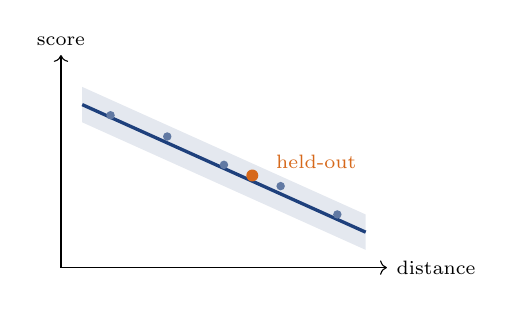
\begin{tikzpicture}[scale=0.9]
        \draw[->] (0,0)--(4.6,0) node[right,font=\scriptsize]{distance};
        \draw[->] (0,0)--(0,3.0) node[above,font=\scriptsize]{score};
        \fill[navy!12] (0.3,2.55) -- (4.3,0.75) -- (4.3,0.25) -- (0.3,2.05) -- cycle;
        \draw[navy,very thick] (0.3,2.3) -- (4.3,0.5);
        \foreach \x/\y in {0.7/2.15,1.5/1.85,2.3/1.45,3.1/1.15,3.9/0.75}
            \fill[navy!70] (\x,\y) circle (1.7pt);
        \fill[burnt] (2.7,1.3) circle (2.4pt);
        \node[burnt,font=\scriptsize,right] at (2.9,1.5) {held-out};
      \end{tikzpicture}\\[-1pt]
      {\scriptsize predicted vs.\ actual, with CIs}
    \end{column}
  \end{columns}
\end{frame}

% ============================================================ IMPLEMENTATION
\section{Implementation}

% ------------------------------------------------------------ roadmap
\begin{frame}{Implementation roadmap --- seven steps, two gates}
  \centering
  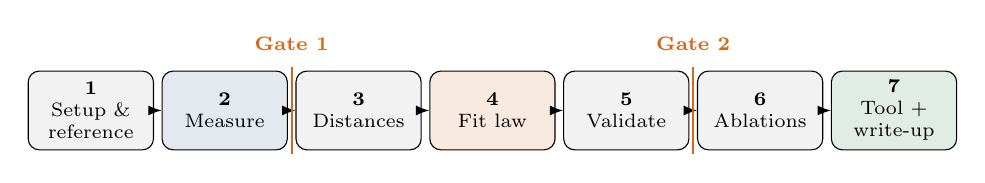
\begin{tikzpicture}[>=Latex, x=1.7cm,
    st/.style={draw,rounded corners,align=center,font=\scriptsize,inner sep=2pt,
               text width=1.45cm,minimum height=1.0cm}]
    \node[st,fill=black!5]  (s1) at (0,0) {\textbf{1}\\Setup \&\\reference};
    \node[st,fill=navy!12]  (s2) at (1,0) {\textbf{2}\\Measure};
    \node[st,fill=black!5]  (s3) at (2,0) {\textbf{3}\\Distances};
    \node[st,fill=burnt!14] (s4) at (3,0) {\textbf{4}\\Fit law};
    \node[st,fill=black!5]  (s5) at (4,0) {\textbf{5}\\Validate};
    \node[st,fill=black!5]  (s6) at (5,0) {\textbf{6}\\Ablations};
    \node[st,fill=forest!14](s7) at (6,0) {\textbf{7}\\Tool +\\write-up};
    \foreach \a/\b in {s1/s2,s2/s3,s3/s4,s4/s5,s5/s6,s6/s7} \draw[->] (\a)--(\b);
    \draw[burnt,thick] ($(s2)!0.5!(s3)+(0,0.55)$)--($(s2)!0.5!(s3)+(0,-0.55)$);
    \draw[burnt,thick] ($(s5)!0.5!(s6)+(0,0.55)$)--($(s5)!0.5!(s6)+(0,-0.55)$);
    \node[burnt,font=\scriptsize\bfseries] at ($(s2)!0.5!(s3)+(0,0.85)$) {Gate 1};
    \node[burnt,font=\scriptsize\bfseries] at ($(s5)!0.5!(s6)+(0,0.85)$) {Gate 2};
  \end{tikzpicture}
  \vspace{0.7em}

  \footnotesize \textcolor{burnt}{\textbf{Gate 1}} (after measurement): are the scores in SA-FARI's SAM\,3
  ballpark?\quad \textcolor{burnt}{\textbf{Gate 2}} (after validation): real out-of-sample signal ---
  else invoke H0 and pivot.
\end{frame}

% ------------------------------------------------------------ step 1
\begin{frame}{Step 1 --- Setup \& the leakage firewall \small(Phase 0)}
  \begin{itemize}
    \item \textbf{Acquire SA-FARI} --- gated annotations (Hugging Face) + public 6\,fps frames (GCS);
          smoke-test SAM\,3 + the official VEval on 1--2 clips.
    \item \textbf{Freeze the seen/unseen reference} --- enumerate train species, locations, and taxonomy,
          then \textbf{assert} the test split is disjoint by species \emph{and} location.
  \end{itemize}
  \vspace{0.3em}
  \begin{block}{The leakage firewall}
    \centering Every distance is later computed against the \frozen{frozen training set only}
    (\texttt{data/reference/*}) --- no test information can enter a feature.
  \end{block}
\end{frame}

% ------------------------------------------------------------ step 2
\begin{frame}{Step 2 --- Measurement: frozen SAM\,3 $\to$ VEval \small(Phase 1)}
  \centering
  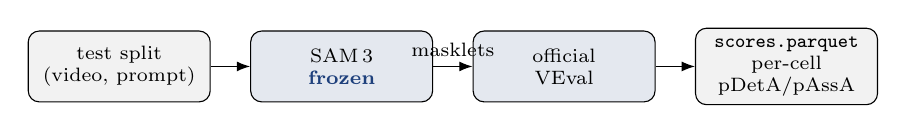
\begin{tikzpicture}[>=Latex,
    box/.style={draw,rounded corners,align=center,font=\scriptsize,inner sep=3pt,text width=2.1cm,minimum height=0.9cm}]
    \node[box,fill=black!5] (t) {test split\\(video, prompt)};
    \node[box,fill=navy!12,right=0.5cm of t] (sam) {SAM\,3\\\frozen{frozen}};
    \node[box,fill=navy!12,right=0.5cm of sam] (ve) {official\\VEval};
    \node[box,fill=black!5,right=0.5cm of ve] (sc) {\texttt{scores.parquet}\\per-cell pDetA/pAssA};
    \draw[->] (t)--(sam); \draw[->] (sam)--(ve) node[midway,above,font=\scriptsize]{masklets}; \draw[->] (ve)--(sc);
  \end{tikzpicture}
  \vspace{0.5em}
  \begin{itemize}\footnotesize
    \item Species-specific prompts (primary) $+$ a generic ``animal'' prompt (robustness); hard negatives kept.
    \item Output $=$ the \textbf{dependent variables}: per-cell \texttt{pDetA}/\texttt{pAssA}/\texttt{pHOTA} $+$ support.
  \end{itemize}
  \centering\footnotesize\textcolor{burnt}{\textbf{Gate 1:} are the scores in SA-FARI's SAM\,3 ballpark?}
\end{frame}

% ------------------------------------------------------------ step 3a
\begin{frame}{Step 3 --- The four label-free distances \small(Phase 2)}
  \centering\footnotesize
  \begin{tabular}{@{}lll@{}}
    \toprule
    \textbf{Distance} & \textbf{computed from} & \textbf{column}\\
    \midrule
    Taxonomic   & LCA tree steps to nearest train species & \texttt{taxonomic\_distance}\\
    Visual      & DINOv2 mask-crop vs nearest prototype    & \texttt{visual\_distance}\\
    Environment & scene embed of masked-out background     & \texttt{environment\_distance}\\
    Temporal    & years to nearest train footage           & \texttt{temporal\_gap}\\
    Familiarity & separability in SAM\,3's own features    & \texttt{familiarity\_proxy}\\
    \bottomrule
  \end{tabular}
  \vspace{0.6em}

  All \textbf{label-free} for the target and computed against the \frozen{frozen train set}.
\end{frame}

% ------------------------------------------------------------ step 3b
\begin{frame}{Step 3 --- Assemble the feature table \small(Phase 2)}
  \centering
  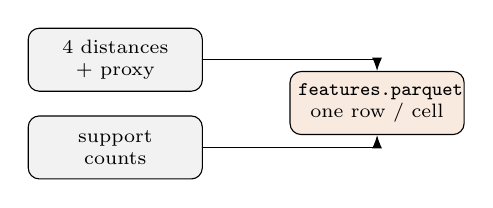
\begin{tikzpicture}[>=Latex,
    box/.style={draw,rounded corners,align=center,font=\scriptsize,inner sep=3pt,text width=2.0cm,minimum height=0.8cm}]
    \node[box,fill=black!5] (d) {4 distances\\+ proxy};
    \node[box,fill=black!5,below=0.3cm of d] (s) {support\\counts};
    \node[box,fill=burnt!14,right=1.1cm of d,yshift=-0.55cm] (f) {\texttt{features.parquet}\\one row / cell};
    \draw[->] (d)-|(f); \draw[->] (s)-|(f);
  \end{tikzpicture}
  \vspace{0.5em}
  \begin{block}{Leakage unit test}
    \centering\footnotesize Swapping the frozen seen set changes the distances \emph{as expected} ---
    no test label enters any column.
  \end{block}
\end{frame}

% ------------------------------------------------------------ step 4
\begin{frame}{Step 4 --- Fit the law \& decompose \small(Phase 3)}
  \begin{itemize}
    \item Model \texttt{pDetA} and \texttt{pAssA} \textbf{separately} with a \textbf{beta / logit-link GLM},
          \emph{weighted by support}, with a \texttt{log(n\_frames)} covariate (so ``rare'' $\ne$ ``far'')
          $\to$ \texttt{outputs/models/*}.
    \item \textbf{Variance partitioning} (dominance/Shapley $+$ VIF) attributes each factor's contribution.
  \end{itemize}
  \vspace{0.3em}
  \begin{block}{The decomposition test}
    \centering\footnotesize Does detection load on \textcolor{forest}{\textbf{species novelty}} and
    association on \textcolor{plum}{\textbf{environment}}? --- the headline contrast.
  \end{block}
\end{frame}

% ------------------------------------------------------------ step 5
\begin{frame}{Step 5 --- Out-of-sample validation \small(Phase 4)}
  \begin{itemize}
    \item \textbf{Grouped CV} --- hold out \emph{whole} species and \emph{whole} locations; predict
          held-out cells from \textbf{distance alone} $\to$ \texttt{cv\_results.parquet} (MAE/RMSE, calibration).
    \item \textbf{Bootstrap CIs} everywhere $+$ the \textbf{predictive-line} figure (predicted vs.\ actual).
  \end{itemize}
  \vspace{0.2em}
  \centering\footnotesize\textcolor{burnt}{\textbf{Gate 2:} real out-of-sample signal? --- else invoke
  \textbf{H0} and pivot to representational probing.}\\[3pt]
  \footnotesize Success $=$ a \emph{validated} predictor, not a higher score.
\end{frame}

% ------------------------------------------------------------ step 6
\begin{frame}{Step 6 --- Ablations \& robustness \small(Phase 5)}
  \begin{itemize}
    \item \textbf{Factor ablations} --- drop each distance and report the $R^2$ / OOS-error change:
          what does each factor contribute?
    \item \textbf{Design \& confound robustness} --- DINOv2 vs.\ CLIP; mask-cropped vs.\ whole-frame;
          species vs.\ generic prompt; $\pm$ the support covariate.
  \end{itemize}
  \vspace{0.3em}
  \centering\footnotesize The detection/association contrast \textbf{holds across variants} --- or its
  limits are documented.
\end{frame}

% ------------------------------------------------------------ step 7
\begin{frame}{Step 7 --- The reliability tool \& write-up \small(Phase 6)}
  \centering
  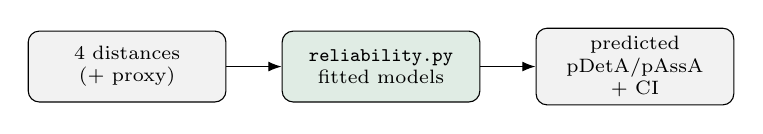
\begin{tikzpicture}[>=Latex,
    box/.style={draw,rounded corners,align=center,font=\scriptsize,inner sep=3pt,text width=2.3cm,minimum height=0.9cm}]
    \node[box,fill=black!5] (in) {4 distances\\(+ proxy)};
    \node[box,fill=forest!14,right=0.7cm of in] (m) {\texttt{reliability.py}\\fitted models};
    \node[box,fill=black!5,right=0.7cm of m] (out) {predicted\\pDetA/pAssA $+$ CI};
    \draw[->] (in)--(m); \draw[->] (m)--(out);
  \end{tikzpicture}
  \vspace{0.5em}
  \begin{itemize}\footnotesize
    \item The deployment \textbf{``will it work here?''} tool: a new (species, place) $\to$ a prediction $+$ interval.
    \item The \textbf{dissertation} --- every claim backed by a repo-generated figure/table.
  \end{itemize}
\end{frame}

% ------------------------------------------------------------ closing
\begin{frame}{Contribution}
  \begin{block}{}
    \centering The deliverable: a \textbf{validated, label-free reliability estimator} for a promptable
    tracker --- and \emph{why} detection and association transfer differently.
  \end{block}
  \vspace{0.6em}
  \centering\small\color{navy}\textbf{Thank you --- questions welcome.}
\end{frame}

\end{document}
